\section{StartupBench}

\begin{table*}[t]
\caption{StartupBench 与现有基准的比较。E2E 表示端到端工作流完成；“逐项评估”表示按准则逐项裁判。\cmark、\xmark 和 \pmark 分别表示完全支持、不支持和部分支持。}
\label{tab:main_stat}
\centering
\resizebox{\textwidth}{!}{
\begin{tabular}{lccccccc}
\toprule
\textbf{基准} &
\textbf{\thead{任务来源}} &
\textbf{\thead{最终\\输出}} &
\textbf{E2E} &
\textbf{\thead{逐项\\评估}} &
\textbf{\thead{过程\\逻辑}} &
\textbf{\thead{开放式}} &
\textbf{\thead{评估\\方法}} \\
\midrule
GAIA \citep{mialon2024gaia} & 人工 & 文本 & \pmark & \xmark & \xmark & \xmark & 规则 \\
OSWorld \citep{xieosworld} & 真实+人工 & 环境状态 & \pmark & \xmark & \xmark & \xmark & 执行 \\
DAComp \citep{lei2025dacomp} & 真实+人工 & 工作空间 & \cmark & \xmark & \xmark & \cmark & 混合 \\
GDPval \citep{patwardhan2025gdpval} & 人工 & 工作成果 & \cmark & \xmark & \xmark & \pmark & 人工 \\
Workspace-Bench \citep{tang2026workspace} & 模拟+人工 & 工作空间 & \cmark & \xmark & \xmark & \cmark & 智能体裁判 \\
OneMillionBench \citep{yang2026onemillion} & 专家编写 & 文本 & \pmark & \xmark & \pmark & \cmark & 模型裁判 \\
Agents' Last Exam \citep{sun2026agents} & 职业引导 & 工作空间 & \cmark & \xmark & \pmark & \pmark & 混合 \\
OfficeQA Pro \citep{opsahl2026officeqa} & 语料库支撑 & 文本 & \xmark & \xmark & \xmark & \xmark & 答案匹配 \\
\midrule
\textbf{StartupBench（本文）} & \textbf{\thead{市场验证\\+专家构建}} & \textbf{工作空间} & \cmark & \cmark & \cmark & \cmark & \textbf{智能体裁判} \\
\bottomrule
\end{tabular}
}
\end{table*}

\begin{figure*}[t]
    \centering
    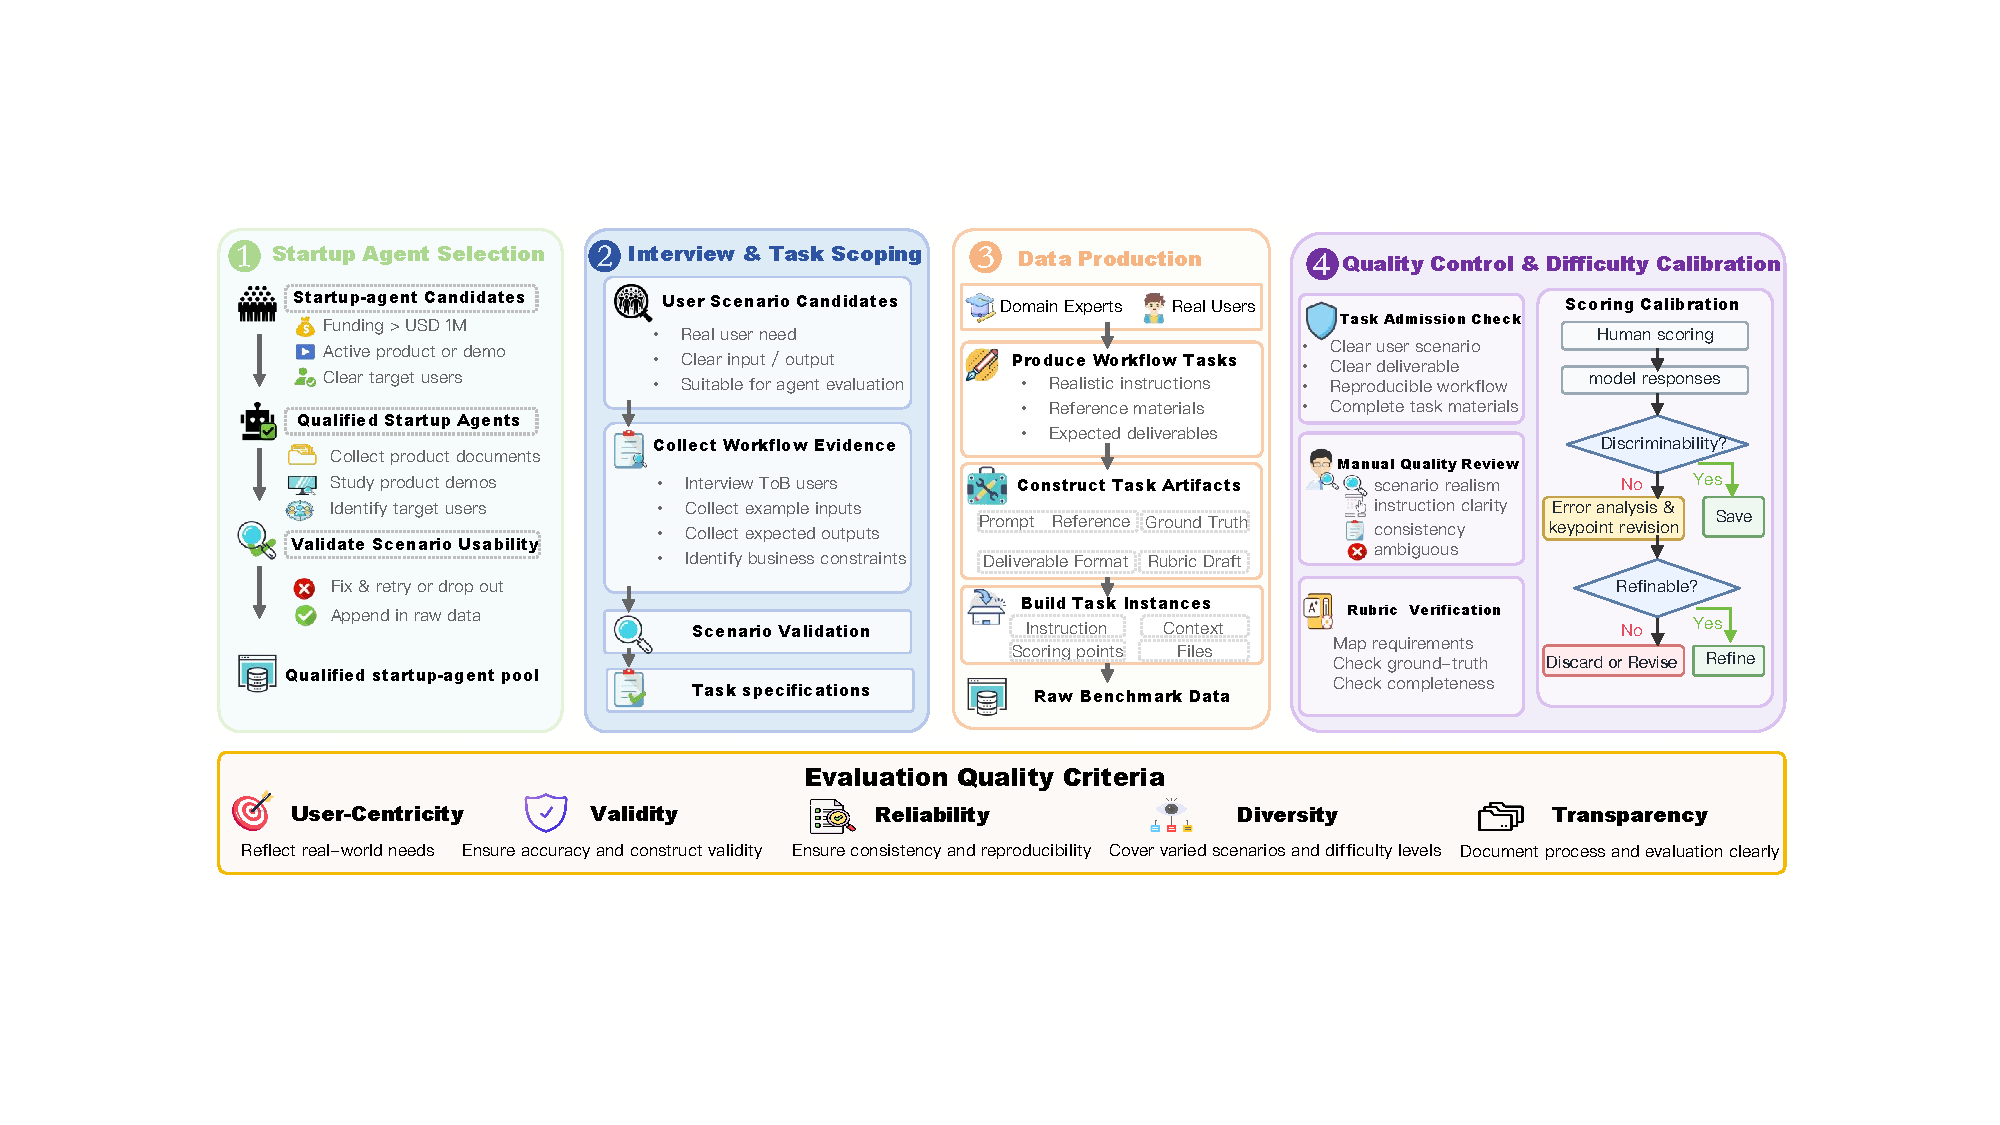
\includegraphics[width=0.99\textwidth]{figures/StartupBench-fig2.pdf}
    \caption{StartupBench 数据构建流程。我们筛选经市场验证的初创企业智能体，收集真实用户工作流，构建任务产物与实例，并通过多阶段审查校准质量和难度。}
    \label{fig:data_workflow}
\end{figure*}

StartupBench 旨在评估模型和智能体能否完成用户已经委派给人工智能产品的现实工作流。实现这一目标所需的数据既要反映真实用户需求，又要支持受控评估。因此，我们要求每项任务都具备真实性、可解答性、可评估性和区分度：任务应源自人工智能产品的实际使用，为有效解法提供充分信息，明确输出要求和评估标准，并保持足够难度，以区分当前不同模型和智能体。

单纯依赖人工任务设计，或直接从产品演示中提取内容，都不足以得到此类数据。前者可控，却可能脱离真实需求；后者真实，却常常缺少上下文、成功标准或可复现的任务说明。因此，我们采用图~\ref{fig:data_workflow} 所示的、由调研和访谈驱动的多阶段流程。首先，我们调研经市场验证的人工智能原生初创企业；随后访谈深度用户，识别使用情境、任务目标和预期交付物；再招募领域专家，把经过验证的场景转化为基准实例；最后从真实性、可解答性、可评估性和具有区分度的难度四方面实施质量控制。

\subsection{数据集构建}

\subsubsection{面向市场验证智能体场景的初创企业调研}
我们首先调研在不同领域构建智能体产品的人工智能原生初创企业。为识别获得市场验证的工作流，我们仅保留融资额超过 100 万美元的初创企业，并要求存在真实采用证据，即付费使用或显著的用户吸引力。融资是市场预期的一项粗略信号，而付费或用户规模证据则表明产品的使用已超出探索性演示。该阶段的输出是供用户访谈使用的候选产品和工作流池。在这一阶段，我们收集了 20 余个初创企业智能体，作为后续阶段的基础。

\subsubsection{用于发现场景与需求的用户访谈}
对于每个候选初创企业产品，我们访谈来自不同领域、使用相应智能体的深度用户，以恢复公开产品描述之外的实际使用情况。访谈旨在获取使用情境、用户目标、输入信息、预期交付物、成功标准和常见约束。我们把这些发现汇总为场景说明和代表性演示案例，作为后续标注阶段的锚点。在这一阶段，我们访谈了 30 多位深度用户，并为每个候选智能体至少收集一个演示案例。

\subsubsection{由专家构建领域任务}
我们以访谈得到的工作流说明和代表性用户场景作为参考或种子任务，招募 50 多位领域专家重构基准任务。在把任务调整为可复现评估实例的同时，专家需保留原始工作流目标、实际约束和预期交付物。专家并非设计合成问题，而是把真实用户请求标准化为能够忠实代表现实专业工作流的基准任务。

每项任务都必须满足三项原则：它必须源自用户会自然委派给人工智能智能体的现实工作请求；必须包含端到端工作流，而非孤立子任务；必须生成具有明确成功标准和细粒度评分细则的具体专业交付物，以便进行客观评估。

为实现标准化评估，每项任务被表示为三元组
\[
\mathcal{T}=(q,\mathcal{E},\mathcal{R}),
\]
其中，$q$ 是描述任务的自然语言用户请求，$\mathcal{E}$ 表示包含完成任务所需全部输入文件和资源的工作空间，$\mathcal{R}=\{(p_i,w_i)\}_{i=1}^{n}$ 是一组带权评估细则，用于评估交付物质量的互补方面。详细任务说明和标注指南见附录~\ref{app:task_construction}。在这一阶段，我们收集了 150 多项候选任务，以供后续质量控制。

\subsubsection{质量控制}
为保证基准的质量与一致性，每项任务都要经历以下多阶段质量控制流程。

\textbf{专家交叉验证。}每项任务至少由另一位领域专家独立审查。审查者验证任务质量的四个方面：（1）任务描述和工作空间的真实性与正确性；（2）重构工作流的忠实度；（3）评估细则的有效性；（4）参考交付物与最终评估协议之间的一致性。详细审查标准见附录~\ref{app:cross_valid}。

\textbf{难度控制。}我们在基准所采用的同一评估框架下，使用若干前沿模型开展试运行，以校准任务难度\footnote{我们从 GPT-5.5、Seed-2.1-Pro 和 GLM-5.1 中随机选择模型执行试运行，目的是构建具有挑战性和区分度的基准，而不是估计模型在自然任务分布上的表现。}。始终能以高质量完成的任务会因区分度有限而被排除。试运行结果还充当额外的质量保障环节：如果失败源于指令含混、工作空间信息不全或评估标准说明不足，而不是任务本身的难度，则相应任务会在纳入前得到修订并再次验证。

\subsection{StartupBench 统计信息}
\textbf{StartupBench} 包含 97 项现实工作流任务，覆盖 6 个一级领域：医疗与健康、金融、法律、商业与管理、STEM 与计算机科学，以及教育与人文学科。这些任务旨在反映现实办公环境中面向交付物的工作流，要求智能体理解任务情境、遵循复杂约束、处理异构文件并生成可用的工作成果。评估时，每项任务平均使用 \textbf{25.3} 条细粒度评分细则，覆盖 \textbf{6 个维度和 3 个重要性层级}，从而能够细致评估复杂的长时程工作流和多样的工作交付物。StartupBench 的领域覆盖和主要输出格式汇总见表~\ref{tab:benchmark_statistics}。

\begin{table}[t]
\centering
\small
\renewcommand{\arraystretch}{1.12}
\begin{threeparttable}
\caption{StartupBench 统计信息。基准包含 97 项现实工作流任务，覆盖六个一级领域，并要求多种交付物格式。}
\label{tab:benchmark_statistics}
\setlength{\tabcolsep}{3pt}
\begin{tabular}{lrr}
\toprule
\textbf{类别} & {\textbf{数量}} & {\textbf{占比（\%）}} \\
\midrule
\rowcolor{gray!8}
\multicolumn{3}{l}{\textit{总体统计}} \\
任务总数 & 97 & 100.0 \\
一级领域 & 6 & \multicolumn{1}{c}{--} \\
\midrule
\rowcolor{gray!8}
\multicolumn{3}{l}{\textit{领域分布}} \\
医疗与健康 & 21 & 21.6 \\
金融 & 18 & 18.6 \\
法律 & 16 & 16.5 \\
商业与管理 & 19 & 19.6 \\
STEM 与计算机科学 & 16 & 16.5 \\
教育与人文学科 & 7 & 7.2 \\
\bottomrule
\end{tabular}
\begin{tablenotes}[flushleft]
\footnotesize
\item \textit{输出格式：}DOCX、XLSX、PPTX、PDF、Markdown、图像和文本类交付物。
\end{tablenotes}
\end{threeparttable}
\end{table}

\subsection{StartupBench 任务的自动评估}
如前所述，StartupBench 中的每项任务都定义为三元组 $\mathcal{T}=(q,\mathcal{E},\mathcal{R})$。给定 $(q,\mathcal{E})$，待评模型会生成一组交付物 $\mathcal{D}$。在评估前，我们构建一个轻量证据视图 $\mathcal{V}(\mathcal{D})$，由提取出的文本内容和渲染页面图像组成，以便在异构产物之间导航；必要时，裁判仍可访问原始文件。

StartupBench 并不依赖单个整体判断，而是通过独立的 AgentJudge 会话逐项评估每条评分细则。大多数任务包含 20 余条细粒度评分细则，覆盖预期交付物的不同方面，包括功能、完整性、格式和领域特定要求。分别评估这些准则，使每一条细则都能得到专门的推理和工具使用，避免不相关评估维度之间相互干扰，同时确保所有要求都被显式检查。最终任务分数由全部细则级评估结果聚合得到。

遵循\textbf{智能体裁判}范式，每条评分细则都由一个轻量智能体而非单次前向传播完成评估。设 $J$ 表示 AgentJudge 使用的裁判提示和评估协议；给定任务说明、交付物、证据视图和目标评分点 $p_i$，裁判同时生成二元判断 $y_i\in\{0,1\}$（表示是否满足该细则）以及文本理由 $e_i$：

\begin{equation}
(y_i,e_i) = \mathrm{AgentJudge}\big(J, q,
\mathcal{D}, \mathcal{V}(\mathcal{D}), p_i\big),
\label{eq}
\end{equation}

最终任务分数通过聚合所有评分细则的加权判断计算：

\begin{equation}
\mathrm{score}(\mathcal{D},\mathcal{T})
= \frac{\sum_{i=1}^{n} w_i y_i}{\sum_{i=1}^{n} w_i}
\in [0,1].
\label{eq2}
\end{equation}

\FloatBarrier
